\documentclass[12pt]{article} % Tamaño de letra
\usepackage[utf8]{inputenc} % Simbolo utf8
\usepackage[light]{antpolt} % Tipo de letra
\usepackage[T1]{fontenc}
\usepackage[spanish]{babel} % Español 
\usepackage[dvipsnames]{xcolor} % Paquete de colores
\usepackage{amsmath} % Paquete de simbolos matematicos
\usepackage{halloweenmath} % Paquete de Halloween
\usepackage{amssymb} % therefore 
\usepackage{amsfonts}  % Alinear
\usepackage{mathtools} 
\usepackage{hyperref} % Hiperreferencias
\usepackage{xurl} % Romper url largos en más líneas
\usepackage{graphicx}
\usepackage{caption} % Paquete para personalizar las captions
\usepackage{tikz} % Dibujos arreglo
\usepackage{graphics}
\usepackage{wrapfig}
\usepackage{subfig}
\usepackage{listings} % Código
\usepackage[shortlabels]{enumitem}
\usepackage{bbm}
\usepackage{multirow, array} % para las tablas
\usepackage{float}
\usepackage{color}
\usepackage{tabularray}
\usepackage{fancyhdr}
\usepackage{pifont}%Simbolos especiales.
\usepackage{fancybox}%Para crear cajas (Notas).
\usepackage[margin=1in]{geometry}
\usepackage[margin=1.1in]{caption}
\pagestyle{fancy}
\fancypagestyle{plain}{
\fancyhf{}\fancyhead[L]{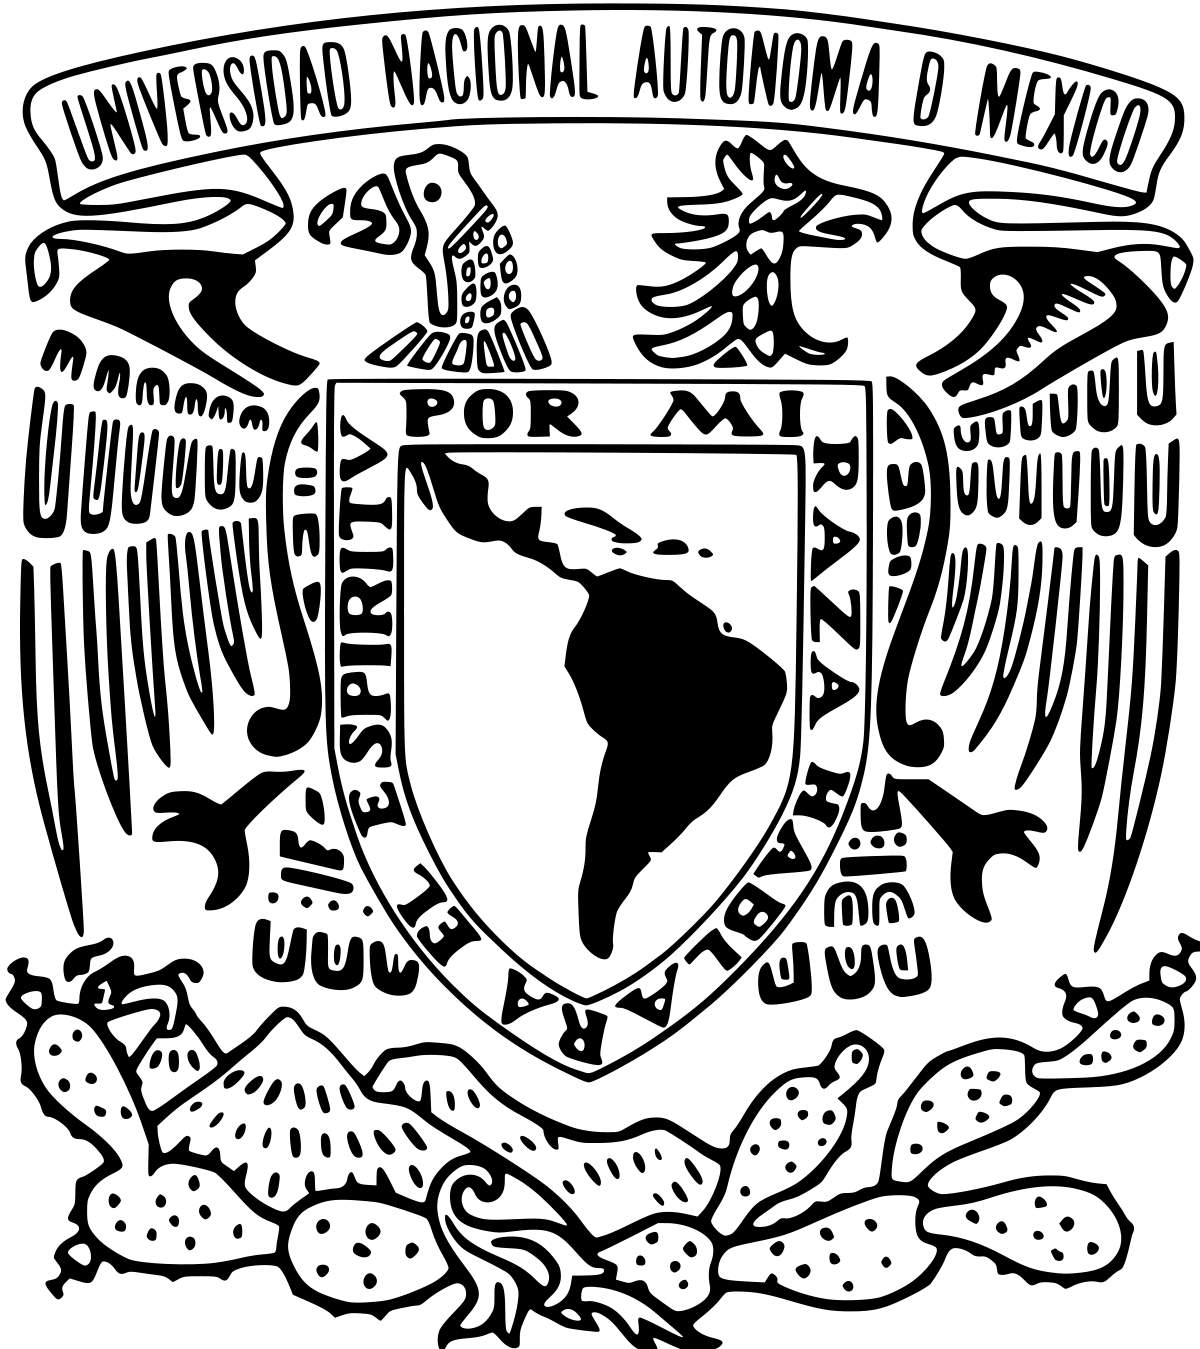
\includegraphics[height=0.5in]{unam.png}}
\fancyhead[R]{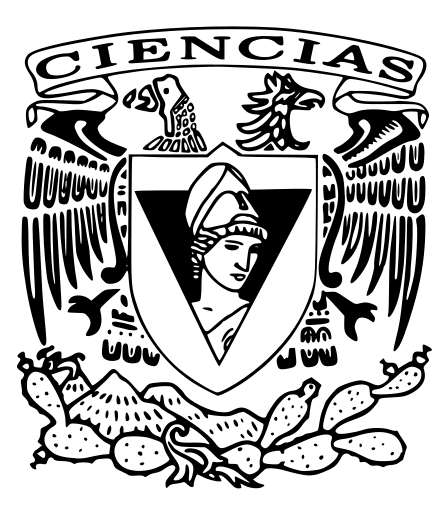
\includegraphics[height=0.5in]{ciencias.png}}
}

%----------[ Declaración Respuesta ]-----------
\usepackage{framed,xcolor} % Color de repuesta

\newenvironment{respuesta}{
    \definecolor{shadecolor}{RGB}{236,236,228}
    \begin{snugshade*}
    \vspace*{2mm}}
    {\vspace*{2mm}
    \end{snugshade*}}

%------------------------------
\definecolor{fondo}{RGB}{234, 236, 238}% Definición del color fondo

\lstset{
    language=Java,
    basicstyle=\ttfamily\footnotesize, % Cambiar el tamaño de la fuente
    keywordstyle=\color{blue},
    commentstyle=\color{OrangeRed},
    stringstyle=\color{ForestGreen},
    numbers=left,
    numberstyle=\tiny,
    stepnumber=1,
    numbersep=5pt,
    backgroundcolor=\color{fondo},
    frame=single,
    rulecolor=\color{black},
    breaklines=true,
    columns=flexible,
    inputencoding=utf8,
    morecomment=[s][\color{purple}]{/**}{*/},
    %morecomment=[l][\color{orange}]{//},
    %literate={\#}{{\#}}1,
    literate={á}{{\'a}}1
             {é}{{\'e}}1
             {í}{{\'i}}1
             {ó}{{\'o}}1
             {ú}{{\'u}}1
             {Á}{{\'A}}1
             {É}{{\'E}}1
             {Í}{{\'I}}1
             {Ó}{{\'O}}1
             {Ú}{{\'U}}1
             {ñ}{{\~n}}1
             {Ñ}{{\~N}}1
             {¿}{{\textquestiondown}}1
             {¡}{{\textexclamdown}}1,
}

\begin{document}
\title{Ejercicios 3: Lista e Iteradores}
\author{Ayudante: Cynthia Lizbeth Sánchez Urbano}
\date{Ejercicios de práctica para Listas e Iterador.}
\maketitle
\section{Lista}
\begin{enumerate}
\item Da 3 ejemplos de listas en la vida cotidiana.
\item Explica que es una lista en estructuras de datos.
\item ¿Qué es un nodo?
\item Si tienes una lista doblemente ligada ¿qué atributos son útiles para el nodo?
\item Observa el siguiente diagrama de una lista con un sólo nodo, y construye una lista con 5 elementos paso a paso, es decir muestra las conexiones que se van creando y el cambio de referencias.
\begin{figure}[H]
\centering
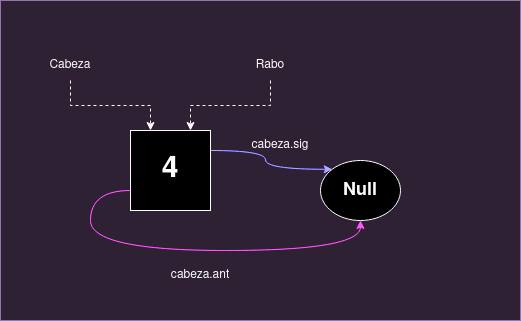
\includegraphics[scale=0.5]{ListaUnNodo.png}
\caption{Lista doblemente ligada con un sólo nodo. Cada nodo tiene referencias a un nodo anterior, a un siguiente, y a un elemento el cual por simpleza se representa dentro del nodo. La lista tiene referencias a el primer elemento (cabeza) y al último (rabo).}
\end{figure}
\item La forma de manejar la lista anterior es identificando un nodo inicial y un nodo final por medio de dos referencias pero existe otra forma de programar la lista, esta segunda forma es por medio de un nodo \textit{centinela}, observa el siguiente diagrama y crea una lista con 5 elementos pero usando este método.
\begin{figure}[H]
\centering
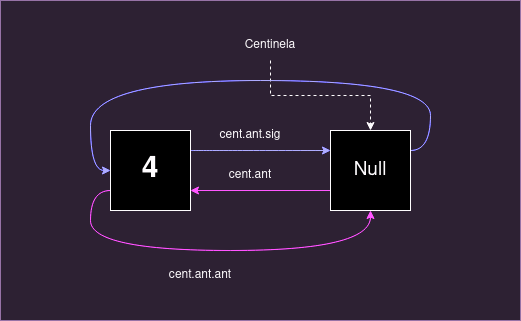
\includegraphics[scale=0.5]{ListaCentinela.png}
\caption{Lista doblemente ligada con un sólo nodo y un nodo especial llamado \textit{centinela}.}
\end{figure}
\item ¿Qué diferencias notas entre estás dos formas de programar la lista? ¿Cuál se te hace más sencilla de comprender?.
\item Toma las listas que dibujaste y elimina 2 elementos de cualquier parte de la lista.
\end{enumerate}
\section{Iterador}
\begin{enumerate}
\item Usando la lista con \textit{centinela} del ejercicio 6 de la sección \textit{Lista} coloca el \textit{iterador} en la posición inicial.
\item Muestra el movimiento que hace el iterador desde la posición inicial hasta que llega al final de la lista, muestra el cambio de referencias y lo que regresan los métodos \textit{hasNext} y \textit{next}.
\item Agrega cualquier elemento a tu lista en una posición intermedia moviéndote con el iterador.
\item Elimina cualquier elemento de una posición intermedia moviéndote con el iterador.
\item Explica con tus propias palabras ¿Qué es el iterador y para que sirve? 
\end{enumerate}
\end{document}